\documentclass[a5paper]{article}
\usepackage[a5paper, top=8mm, bottom=8mm, left=8mm, right=8mm]{geometry}

\usepackage{polyglossia}
\setdefaultlanguage[babelshorthands=true]{russian}

\usepackage{fontspec}
\setmainfont{FreeSerif}
\newfontfamily{\russianfonttt}[Scale=0.7]{DejaVuSansMono}

\usepackage[font=scriptsize]{caption}

\usepackage{amsmath}
\usepackage{amssymb,amsfonts,textcomp}
\usepackage{color}
\usepackage{array}
\usepackage{hhline}
\usepackage{cite}
\usepackage{verse}

\usepackage[hang,multiple]{footmisc}
\renewcommand{\footnotelayout}{\raggedright}

\PassOptionsToPackage{hyphens}{url}\usepackage[xetex,linktocpage=true,plainpages=false,pdfpagelabels=false]{hyperref}
\hypersetup{colorlinks=true, linkcolor=blue, citecolor=blue, filecolor=blue, urlcolor=blue, pdftitle=1, pdfauthor=, pdfsubject=, pdfkeywords=}

\usepackage{tabu}

\usepackage{graphicx}
\usepackage{indentfirst}
\usepackage{multirow}
\usepackage{subfig}
\usepackage{footnote}
\usepackage{minted}

\sloppy
\pagestyle{plain}

\title{Проектирование распределённых приложений, технические вопросы}
\author{Юрий Литвинов\\\small{y.litvinov@spbu.ru}}
\date{07.12.2021}

\begin{document}

\maketitle
\thispagestyle{empty}

\section{Введение}

Подавляющее большинство современных приложений в той или иной степени распределённые. Начиная от простых веб-сайтов, где распределённость сводится к наличию клиента, работающего в браузере или на мобильном телефоне, и простой серверной части, заканчивая огромными распределёнными системами из сотен микросервисов, распределёнными базами данных и системами распределённых высокопроизводительных вычислений типа Apache Spark. При этом при проектировании распределённых приложений следует учитывать массу факторов, связанных с их распределённой структурой: независимые отказы, проблемы согласованности данных, горизонтального масштабирования и т.д. Поэтому проектированию распределённых приложений в этом курсе уделяется особое внимание.

Итак, распределённая система --- это приложение, компоненты которого находятся в компьютерной сети и взаимодействуют друг с другом через обмен сообщениями. Как правило, все компоненты так или иначе работают с какими-то общими ресурсами, которые так же хранятся где-то в сети. Собственно, распределённость и нужна обычно для того, чтобы предоставлять доступ к общим ресурсам сразу нескольким пользователям либо одному пользователю, но с разных устройств, либо организовать эффективную распределённую обработку и хранение информации. При этом есть принципиальные отличия распределённых систем от <<обычных>> приложений (хотя сейчас стоило бы распределённые системы называть обычными).

\begin{itemize}
    \item Распределённые системы принципиально параллельны, и по-другому никак не сделать. Причём, это не <<обычная>> многопоточная параллельность, а многопроцессная, когда компоненты системы не имеют доступа к общей памяти\footnote{В подавляющем большинстве случаев. Есть системы с распределённой памятью, но они очень редки.}, при этом ещё расходы на коммуникацию между процессами весьма значительны.
    \item Каждый компонент распределённой системы --- это отдельный процесс, который может работать или не работать по тем или иным причинам независимо от остальных компонентов (так называемые <<независимые отказы>>). Плюс к тому сеть принципиально ненадёжна, поэтому присутствуют ещё временные отказы, связанные со сбоями работы сети.
    \item Опять-таки по самой природе сети невозможно установить единую для системы последовательность событий (то есть в системе нет единого времени), что может быть критично для поддержания целостности данных. Пакеты могут приходить в разном порядке, в разное время разным адресатам, или не приходить вообще, причём это не ошибка, а вполне нормальная ситуация. Так что два разных компонента могут видеть действия пользователей в совершенно разном порядке, что приводит к проблемам гонок гораздо большего масштаба, чем это обычно случается в многопоточном программировании, и требует гораздо больших усилий, если с этим надо бороться.
\end{itemize}

Вообще, есть даже известный список заблуждений, которые имеют разработчики <<десктопных>> систем, только-только погружающиеся в программирование распределённых систем\footnote{Страница в Википедии: \url{ https://en.wikipedia.org/wiki/Fallacies_of_distributed_computing} (дата обращения: 13.10.2021).}:

\begin{itemize}
    \item сеть надёжна --- нет, она даже при обычном функционировании может терять соединение относительно надолго, поэтому любое сетевое приложение должно уметь восстанавливаться после сетевых ошибок и быть готовым к потере связи с любым из компонентов;
    \item задержка при передаче нулевая, поэтому можно взять монолитное приложение, распилить его на веб-сервисы и в цикле от одного до миллиона слать к веб-сервису запросы;
    \item пропускная способность бесконечна, поэтому идея гонять между сервисами туда-сюда гигабайтные файлы не совсем безумна;
    \item сеть защищена и уж ваш-то сервис никто не будет пытаться взломать --- на самом деле не надо даже злого умысла, нанести ущерб может давно забытый червь, всё ещё влачащий жалкое существование где-то в локалке;
    \item топология сети не меняется, так что если хорошо работало вчера, то будет работать и завтра -- но тут уборщица случайно выдёргивает сетевой кабель из маршрутизатора;
    \item администрирование сети централизовано, поэтому если такой-то порт открыт в локальной сети вашей компании, то открыт и у всех остальных --- однако автор как-то разрабатывал ПО для школ, там обычный пользователь не имеет прав даже на запись на диск;
    \item расходы на передачу данных равны нулю, поэтому можно не закладывать в смету проекта расходы на сетевое оборудование, плату за трафик и аренду инфраструктуры;
    \item сеть однородна, так что можно рассчитывать на одинаковую повсюду среду передачи с одинаковыми физическими свойствами каналов связи --- ни у кого из ваших пользователей нет мобильного или спутникового интернета, например.
\end{itemize}

\section{Архитектура распределённых систем}

Из введения могло сложиться впечатление, что разработка распределённых систем --- чрезвычайно сложная задача. Однако уже успел сложиться набор практик, типовых архитектур и технологий, который при аккуратном использовании позволяет решить многие из проблем и сделать сетевую разработку доступной даже школьникам. Начнём рассмотрение мы с самого низкого уровня, с технологий коммуникации в сетевых приложениях, а в следующей версии рассмотрим более <<архитектурные>> вопросы.

Для начала рассмотрим, как вообще можно организовать взаимодействие компонентов в распределённой системе. Каждый компонент является независимым приложением, работает как отдельный процесс, но должен активно общаться с остальными компонентами системы. Возможны следующие варианты того, как это устроить.

\begin{itemize}
    \item Межпроцессное взаимодействие средствами ОС, если компоненты расположены физически на одном устройстве. Например, взаимодействие через пайпы или именованные пайпы (в Linux такая схема работы очень популярна, но Windows так тоже умеет), через общие файлы (как правило, плохая идея, потому что есть пайпы --- те же файлы, но без долгой записи на диск). Так может быть организована связь с СУБД, если бизнес-логика и СУБД находятся на одной машине, и это может быть в разы эффективнее, чем сетевое соединение. На самом деле, это не очень распределённый сценарий работы, так что дальше мы его рассматривать не будем.
    \item Механизмы удалённого вызова по сети: простые протоколы <<запрос-ответ>> (например, так работают REST-сервисы, про которые попозже), удалённые вызовы процедур (RPC, Remote Procedure Calls), удалённые вызовы методов (RMI, Remote Method Invocation --- так работают веб-сервисы). Такие механизмы предполагают наличие сетевого соединения (хотя оно вполне может быть с сервером на той же машине --- для универсальности кода и гибкости деплоя, хотя и медленнее и хуже, чем более специализированные для такого случая способы). Кроме того, чаще всего большая часть работы по организации коммуникаций может быть реализована один раз в некоем middleware (например, RPC реализуют известные инструменты gRPC, Apache Thrift, ZeroC ICE), причём такие инструменты поддерживают кодогенерацию клиентской и серверной стороны коммуникаций, так, чтобы прикладной программист мог пользоваться удалёнными методами так же, как и локальными.
    \item Механизмы неявного взаимодействия: распределённая общая память (требует суровой поддержки и очень редка, так что далее не рассматривается), очереди сообщений и разные архитектуры на основе очередей или каналов, куда можно посылать сообщения и откуда сообщения можно читать. Отличаются от механизмов удалённого вызова тем, что вызывающий не знает ничего о вызываемом и отправляет запрос некоему посреднику в надежде, что он кем-то будет обработан. Запросы часто хранятся, так что доставка адресату может быть отложенной --- компонентам не обязательно находиться онлайн одновременно. Самые простые такие архитектуры могут просто связывать клиент и сервер очередью (например, модель <<издатель-подписчик>>, где кто-то кидает в очередь события, а кто-то подписывается на те из них, что ему интересны), также распространены и общие шины, куда могут писать и откуда могут читать многие участники взаимодействия. Для таких вещей тоже есть готовая инструментальная поддержка, например, мы рассмотрим RabbitMQ как одну из самых популярных реализаций очереди сообщений. Есть целые фреймворки, построенные вокруг неявного взаимодействия, например, Robot Operating System\footnote{Домашняя страница ROS: \url{https://www.ros.org/} (дата обращения: 13.10.2021).}, которая архитектурно интересна и довольно типична для распределённых приложений, но мы её не рассмотрим из-за нехватки времени.
\end{itemize}

Вне зависимости от варианта организации коммуникации возможны также и разные варианты размещения компонент приложения в сети. Наиболее типичным является разбиение сервисов по нескольким серверам:

\begin{center}
    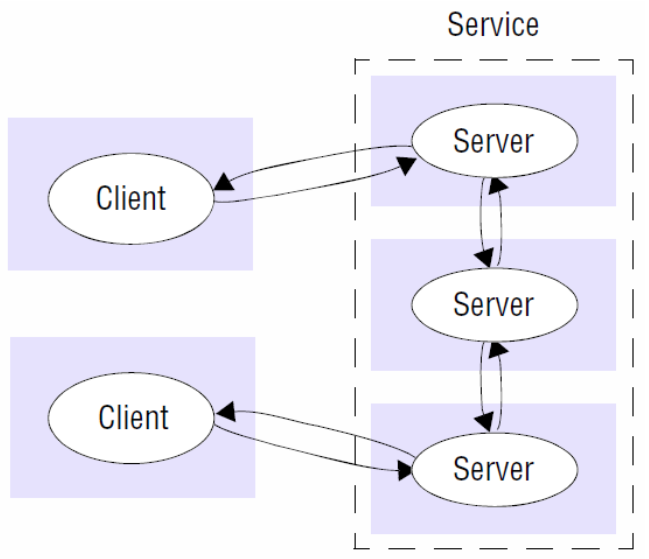
\includegraphics[width=0.45\textwidth]{clientServer.png}
\end{center}

Клиентская часть приложения общается с одним или несколькими сервисами, предоставляющими <<точку входа>> в распределённое приложение --- если это веб-приложение, они же отдают клиенту html-ки и скрипты, которые и составляют клиентскую часть (в том числе по соображениям безопасности --- браузеры сильно ограничивают запросы ко всему, кроме URL, с которых получили страницу). Эти сервисы, в свою очередь, могут вызывать другие сервисы, составляющие приложение, и вместе решать задачу. В больших приложениях таких сервисов могут быть десятки, а то и сотни. В реальной жизни используется некоторая дополнительная инфраструктура --- балансировщики нагрузки, автоматическое масштабирование, системы мониторинга и т.д.

Альтернативными (в каком-то смысле) вариантами размещения являются <<мобильный код>> и <<мобильный агент>>. Мобильный код --- это когда клиент при подключении к серверу получает себе для исполнения код, который делает большую часть содержательной работы на стороне клиента (как правило, в браузере). Так устроены многие современные веб-приложения, например, Google Docs, хотя конкретно в случае Google Docs за мобильным кодом стоит также и большая серверная инфраструктура. Мобильный агент --- это полноценная программа, скачиваемая клиентом и исполняемая на стороне клиента. Используются в основном в peer-to-peer распределённых вычислениях и различных приложениях <<интернета вещей>>, когда данных для обработки много, и доставить код к данным проще, чем собирать данные с оконечных устройств на серверах для обработки.

Также может активно использоваться кеширование, для экономии времени и сетевого трафика при доставке либо данных, либо кода до клиента. Для чего тоже есть широко распространённые готовые решения, например, Redis\footnote{REmote DIctionary Server, \url{https://redis.io/} (дата обращения: 13.10.2021).}.

\section{RPC}

Рассмотрим теперь конкретные технологии организации сетевого взаимодействия компонентов, и начнём с RPC/RMI-инструментов. Все системы удалённого вызова принципиально устроены как на рисунке:

\begin{center}
    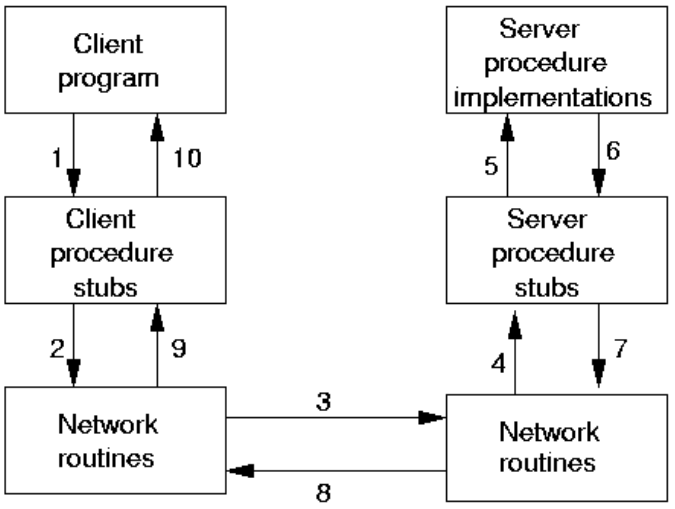
\includegraphics[width=0.45\textwidth]{rpc.png}
\end{center}

ПРи этом программисты пишут только самые верхние блоки --- клиентскую программу и реализации процедур на сервере, которые мы хотим вызывать через RPC. Ещё нужно описать интерфейс сервера --- как правило, в каком-то языконезависимом формате, по которому потом RPC или RMI-система сгенерирует \emph{заглушки} для клиента и для сервера на нужном языке программирования. Клиентские заглушки внешне выглядят как обычный класс, с методами, которые должны быть у соответствующего класса на сервере. Клиентский код может создать заглушку, передать ей каким-то образом адрес и порт сервера (возможно, параметры, нужные для аутентификации/авторизации), и начать вызывать методы как обычно. При этом сгенерированный в заглушке код берёт на себя установление и поддержание сетевого соединения, сериализацию/десериализацию параметров и возвращаемых результатов, передачу данных по сети (используя сетевой стек операционной системы). На сервере всё происходит в обратную сторону --- серверная заглушка, получая сетевой запрос, десериализует параметры, находит и вызывает нужный метод, написанный автором сервера, сериализует ответ, отправляет его по сети обратно.

Светлая цель авторов первых RPC-систем --- чтобы удалённые вызовы были максимально похожи на обычные, так что любой человек, который в состоянии вызвать метод класса, мог бы писать сетевые приложения. При разработке с использованием RPС-систем можно было не думать, на какой машине на самом деле находится тот или иной объект (то, что называется <<location and access transparency>>) --- если на нашей, вызов выполняется как обычно, локально. Если на другой, RPC позаботится обо всех технических деталях и вызов будет выглядеть как обычный.

Однако современная архитектурная мысль сходится к тому, что всё не так просто и различать локальные и удалённые вызовы всё-таки надо. Удалённые вызовы уязвимы к отказам, причём это могут быть отказы самого сервиса (например, он падает при обработке запроса из-за разыменования нулевого указателя) или отказы сети (например, пакет с запросом был потерян перегруженным роутером). И если первый вид отказов критичен для приложения, и надо выдать диагностику клиенту и аккуратно завершить работу, то второй вид отказов надо просто уметь обрабатывать. Есть известная стратегия обработки сетевых отказов --- <<exponential backoff>>, когда мы повторяем запрос, каждый раз увеличивая вдвое время ожидания между попытками, пока запрос не будет успешно исполнен или количество попыток не истечёт. Это позволяет быстро уменьшить частоту запросов, так что если причиной отказа стала перегруженная сеть или перегруженный сервер, общая нагрузка снизится и приложение восстановит работу.

Кроме того, сетевой вызов, в отличие от локального, не мгновенен. Поэтому очень желательно проектировать сетевые вызовы асинхронными, с возможностью отмены операции со стороны клиента. Для локальных вызовов так тоже делают, но только если они могут быть реально длительными, в сетевом же случае каждый запрос может остановить клиент на несколько секунд, если выполняется не асинхронно.

Поэтому многие рекомендуют явно маркировать удалённые вызовы как удалённые, придумав схему именования и используя её консистентно в стиле кодирования. Хотя довольно мало кто так делает на самом деле --- всё-таки удобство RPC-систем и <<прозрачность>> сетевых вызовов весьма привлекательны. Стоит также указывать явно семантику исполнения операции: \emph{at least once} (должна быть исполнена, но спокойно относится к повторам --- как правило, это запросы, не меняющие состояния сервера), \emph{at most once} (операция может быть исполнена не более одного раза, но потеря запроса допустима --- применяется в ситуациях, когда клиент может легко понять, что операция не исполнена, и повторить её), \emph{exactly once} (операция должна быть исполнена обязательно и ровно один раз --- эту семантику труднее всего реализовать в условиях ненадёжной сети, но зачастую необходимо).

RMI (Remote Method Invocation) --- это тот же RPC, но знающий об объектно-ориентированном программировании. Поскольку большинство современных систем пишутся в объектно-ориентированном стиле, многие веб-сервисы реализуются с использованием той или иной RMI-технологии (в большей или меньшей степени RMI). Почему не все --- RPC-системы легковеснее, проще в использовании, быстрее и надёжнее в работе, так что для несложных сервисов предпочтительнее. А поскольку нынче в моде микросервисные архитектуры, где все сервисы должны быть как можно более несложными, RPC-системы популярны. RMI, однако же, более приятны при разработке больших информационных систем: они умеют исключения, иногда умеют распределённые ссылки на объекты (то есть в качестве идентификатора объекта используется не указатель на него в памяти, поскольку память на разных машинах разная и указатели бесполезны, а некий <<глобальный>> идентификатор), ссылки можно передавать как параметры и возвращать как результаты:

\begin{center}
    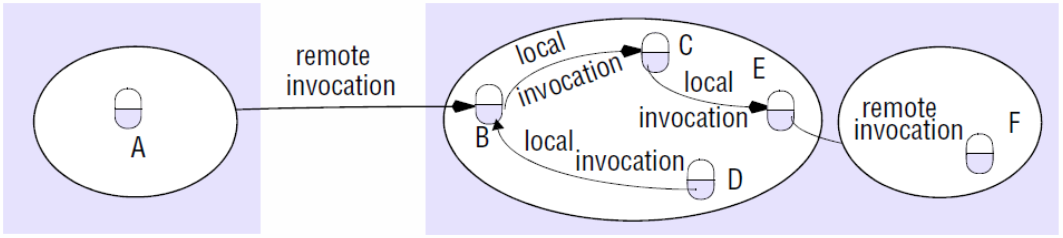
\includegraphics[width=0.8\textwidth]{remoteCalls.png}
\end{center}

Некоторые продвинутые RMI-системы умеют даже распределённую сборку мусора, но автору не приходилось с такими работать.

\subsection{protobuf}

Рассмотрим типичный и активно использующийся в индустрии пример RPC-системы --- Google gRPC. Но поскольку gRPC использует в качестве протокола сериализации протокол от Google, который называется protobuf, сначала кратко рассмотрим его.

Google Protocol Buffers (более известный как protobuf) --- это бинарный формат сериализации произвольных данных. Разработан для внутренних нужд сервисов Google, с целью сэкономить трафик и время передачи. Ближайшие аналоги (XML и JSON) хранят данные в текстовом виде, что хорошо в плане отладки, поскольку они человекочитаемы, но не очень хорошо в плане эффективности передачи или места на диске. protobuf же сериализует данные в хитрый бинарный формат (см. \url{https://developers.google.com/protocol-buffers/docs/encoding}, особого внимания заслуживает способ хранения целых чисел --- Base 128 Varints), что позволяет, по их заявлениям, хранить данные в среднем в 10 раз компактнее формата XML. За это, естественно, надо платить --- protobuf-сообщение не содержит в себе практически никакой информации о своей структуре, передаются только номера полей и значения, при этом чтобы однозначно разобрать сообщение, надо знать типы полей, описанные отдельно.

Это самое отдельное описание --- декларативное описание структуры сообщения в файле .proto, по которому генерируется код для чтения/записи сообщения. Вот пример .proto-файла:

\begin{minted}{protobuf}
syntax = "proto3";

message Person {
    string name = 1;
    int32 id = 2;
    string email = 3;
}
\end{minted}

Версий protobuf бывает две --- proto2 и proto3, с небольшими синтаксическими отличиями, в реальности используются обе (подробности про отличия --- см. в документации). Инструменты поддерживают обе версии протокола, но первой строкой надо указывать версию протокола. Дальше идёт одно или несколько описаний форматов сообщений (в нашем примере --- Person). Сообщения состоят из полей, у каждого поля есть имя, тип и номер. Номера нужны для поддержки изменений в формате записи --- сервер, получив сообщение с незнакомыми полями, может их спокойно проигнорировать. Номера полей есть в любой подобной технологии (например, Apache Thrift описывает формат передачи похожим образом), поскольку протоколы связи имеют свойство эволюционировать, и поддержание обратной совместимости в распределённых приложениях весьма важно.

Ещё protobuf умеет типы-перечисления, массивы/списки (с помощью ключевого слова repeated), вложенные сообщения, импорт сообщений из других файлов, даже что-то вроде вариантных записей (с помощью ключевого слова oneof). В общем, довольно развитый мини-язык программирования для описания данных.

На .proto-файлы во время сборки приложения напускается генератор protoc, который генерирует код под целевой язык программирования. Например, для Java он генерирует класс, представляющий сообщение, и строитель (паттерн <<Строитель>>), который позволяет удобно сообщение сформировать. Поддерживать эти файлы не надо, и даже смотреть на них не надо, они перегенерятся после каждой сборки. В клиентском коде пользоваться ими можно, например, вот так:

\begin{minted}{java}
Person john = Person.newBuilder()
    .setId(1234)
    .setName("John Doe")
    .setEmail("jdoe@example.com")
    .build();
output = new FileOutputStream(args[0]);
john.writeTo(output);
\end{minted}

Builder-у передаются значения полей, дальше методом build() он делает собственно сообщение, у которого есть метод writeTo, принимающий поток, куда надо записать байтовый массив с сериализованным сообщением. Обычно это сетевой поток, но никто не мешает писать protobuf-сообщения на диск (это вполне валидный и весьма компактный формат сохранения), или вообще куда угодно.

protoc обычно подключается как дополнительный компилятор средствами системы сборки. Например, для gradle и maven есть плагины, укачивающие при сборке protoc как maven-пакет, запускающие его на все .proto-файлы, и подключающие результат генерации как обычные Java- или Kotlin-файлы в проект перед запуском обычного компилятора. То есть настройка процесса сборки --- это просто скопировать несколько строк в свой файл с конфигурацией сборки, ничего качать и устанавливать не нужно. Более-менее аналогично оно работает и для других языков (в C++, правда, так и нет пока стандартного пакетного менеджера, там protoc подключить посложнее). Поддерживаются языки Java, Python, Kotlin, Objective-C, C++, Go, Ruby, C\#, Dart.

\subsection{gRPC}

\end{document}